\documentclass{article}
\usepackage{graphicx} % Required for inserting images
\usepackage[a4paper,margin=2.5cm]{geometry}
\usepackage{amsmath}
\usepackage{float}
\usepackage{xcolor}
\usepackage{listings}
\usepackage{caption}
\usepackage{subcaption}
\usepackage{xparse}
\usepackage{hyperref}
\usepackage{amssymb}
\usepackage{verbatim}
\usepackage{fancyhdr}
\pagestyle{fancy}
\usepackage{xspace}
\cfoot{}
\lfoot{SMOS, Universitat Politècnica de Catalunya, year 2023-24}
\rfoot{\thepage}

\definecolor{codegreen}{rgb}{0,0.6,0}
\definecolor{codegray}{rgb}{0.5,0.5,0.5}
\definecolor{codepurple}{rgb}{0.58,0,0.82}
\definecolor{backcolour}{rgb}{0.95,0.95,0.92}

\lstdefinestyle{mystyle}{
    backgroundcolor=\color{backcolour},   
    commentstyle=\color{codegreen},
    keywordstyle=\color{magenta},
    numberstyle=\tiny\color{codegray},
    stringstyle=\color{codepurple},
    basicstyle=\ttfamily\footnotesize,
    breakatwhitespace=false,         
    breaklines=true,                 
    captionpos=b,                    
    keepspaces=true,                 
    numbers=left,                    
    numbersep=5pt,                  
    showspaces=false,                
    showstringspaces=false,
    showtabs=false,                  
    tabsize=2
}
\lstset{style=mystyle}

\title{\textbf{Metropolis Algorithm}}
\author{Student: Giacomo Calabria}
\date{}

\begin{document}
\maketitle

\section*{Introduction}
Using importance sampling it is possible to decrease the variance in estimation of the value of an integral. We consider the following problem of optimisation: finding the global optimum of a given function. Generally, the function can have a larger number of variables/degrees of freedom and an Newton steepest descent method can be inefficient as the number of local minimum can be large. A better efficiency can be obtained if the jump over barriers is allowed, so the deepest wells have larger probability of being considered.
\begin{figure}[H]
    \centering
    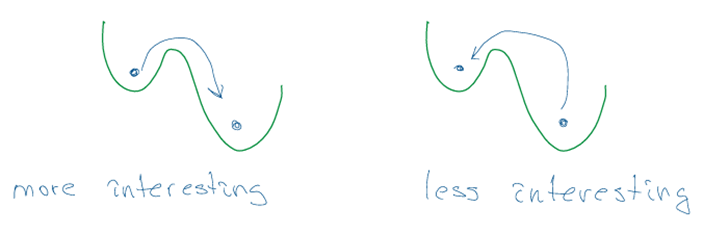
\includegraphics[width=0.5\linewidth]{image.png}
    \label{fig:enter-label}
\end{figure}
\section{Two-dimensional Thompson atomic model}
We wanna simulate a system consisting of $N$ Coulomb charges in a two-dimensional harmonic trap where the potential energy is given by:
\begin{equation}
    E_{pot}=\sum_{i=1}^N{\frac12m\omega^2r_i^2+\sum_{i<j}^N{\frac{q^2}{\left|\mathbf{r}_i-\mathbf{r}_j\right|}}}
\end{equation}
Using some convention in units and dimensionless variables. We can write the potential energy as:
\begin{equation}
    \Tilde{E}_{pot}=\sum_{i=1}^N{\tilde{r}_i^2+\sum_{i<j}^N{\frac{1}{\left|\mathbf{r}_i-\mathbf{r}_j\right|}}}
\end{equation}
In two dimensions, it becomes
\begin{equation}
    \Tilde{E}_{pot}=\sum_{i=1}^N{(x_i^2+y_i^2)+\sum_{i<j}^N{\frac{1}{\sqrt{(x_j-x_i)^2+(y_j-y_i)^2}}}}
\end{equation}
Theoretically, for $N$ particles, the total energy can be approxximated as:
\begin{equation}
    \Tilde{E}=\left(N^{2/3}-1\right)\cdot N2^{1/3}
\end{equation}
This formulation was implemented in Python with the following code
\begin{lstlisting}[language=Python]
def potential(N, R):
    E = 0
    for i in range(N):
        E += (R[i,0]**2 + R[i,1]**2)
        for j in range(i+1,N):
            E += 1/np.sqrt((R[i,0]-R[j,0])**2 + (R[i,1]-R[j,1])**2)
    return E
\end{lstlisting}
It has been tested with some fixed configuration, eg $N=2,r=0.5\rightarrow E_{pot}=1.5$.\\
We wanna use the classical Monte Carlo method and the annealing method to find the minimal energy configuration.
\section{Annealing method}
The metropolis algorithm can be implemented by calculating
\begin{equation}
    \exp{\left\{-\frac{E(\mathbf{R}')-E(\mathbf{R})}{T}\right\}}
\end{equation}
where $T$ is an artificial temperature.\\\\
This formulation was implemented in Python with an simple routine
\begin{lstlisting}[language=Python]
def MaxBoltz(dE, T):
    return math.exp(-(dE)/T)
\end{lstlisting}
\section{Metropolis algorithm}
Now we describe briefly the steps of the Metropolis algorithm; starting from a random configuration of $N$ charges.
\begin{enumerate}
    \item Generate a new/trial position $R_i'$, from the present one $R_i$
    \item Populate the weight $w = p(R_i')/p(R_i)$
    \item Decide the acceptance of the new proposal position, based on the likelihood:\\
    generate a random uniform number $0<u<1$
    \begin{enumerate}
        \item If $int(w+u)>0$ then is \textbf{accepted} and move to the new position $R_{i+1}=R_i'$
        \item If $int(w+u)=0$ then is \textbf{rejected} and stay in the actual position $R_{i+1}=R_i$
    \end{enumerate}
    \item Repeat
\end{enumerate}
We deploy both Local and Global move of the charges. 
\begin{itemize}
    \item Local move: a charges is selected randomly to be moved by a random displacement.
    \item Global move: involves all charges, are moved by a random displacement.
\end{itemize}
The new trail configuration is accepted or rejected based on Metropolis criterion. Also each trail configuration is always accepted if the potential energy is lower than the previous configuration.\\\\
The amplitude of the displacement $\Delta t$ is selected in order to obtain an acceptance ratio close to 50\%. The displacement is done as:
\begin{equation}
    \begin{cases}
        x'=x+\xi_x&\xi_x=(u_x-1/2)\Delta t\\
        y'=y+\xi_y&\xi_y=(u_y-1/2)\Delta t
    \end{cases}
\end{equation}
with $0<u<1$ being from a uniformly distributed random variable.
\begin{lstlisting}[language=Python]
def MoveOneParticle(N,R,T,dt):
    R_new = R.copy()
    # Random choice of one charge to move
    i = np.random.randint(N)
    # Do a random displacement
    R_new[i] += np.random.rand(2) * dt - dt/2
    # Potential energy difference calculation
    dE = potential(N, R_new) - potential(N, R)
    # Acceptance or rejection of the new position based on the metropolis algorithm
    if dE < 0:
      return R_new
    else:
      p_acc = MaxBoltz(dE, T)
      if np.random.rand() < p_acc:
        return R_new
      else:
        return R
\end{lstlisting}
\clearpage
\begin{lstlisting}[language=Python]
def MoveAllParticles(N,R,T,dt):
    R_new = R.copy()
    # Do a random displacement
    for i in range(N):
      R_new[i] += np.random.rand(2) * dt - dt/2
    # Potential energy difference calculation
    dE = potential(N, R_new) - potential(N, R)
    # Acceptance or rejection of the new position based on the metropolis algorithm
    if dE < 0:
      return R_new
    else:
      p_acc = MaxBoltz(dE, T)
      if np.random.rand() < p_acc:
        return R_new
      else:
        return R
\end{lstlisting}
Monte Carlo with annealing procedure, on each step the temperature is lowered by a tiny fraction at each iteration $T'=T\cdot\delta_T$.\\\\The annealing procedure is repeated in a number of times in order to obtain the optimal configuration at the lowest energy.
\begin{lstlisting}[language=Python]
N = 5   # Total number of charges
T0 = 10  # Starting temperature
Tf = 0.01  # Final temperature
dt = 0.5  # Displacement amplitude
steps_per_T = 10000
cooling_rate = 0.995
count = math.ceil(math.log(Tf / T0) / math.log(cooling_rate))

while T > Tf:
  pbar.update()
  for _ in range(steps_per_T):
    R = MoveOneParticle(N, R, T, dt)
  for _ in range(steps_per_T):
    R = MoveAllParticles(N, R, T, dt)
  T *= cooling_rate
  Temp[i] = T
  E[i] = potential(N, R)
  i += 1
\end{lstlisting}
\clearpage
\section{Results - \textit{N=5}}
We simulate a system of $N=5$ charges with the following parameters:
\begin{itemize}
    \item Start temperature: $T_0=10$
    \item Final temperature: $T_f=0.01$
    \item Temperature step: $\delta_T=0.995$
    \item Displacement amplitude: $\Delta t=0.5$
    \item Monte Carlo iterations for each temperature step: $N_{iter}=10000$
\end{itemize}
For $N=5$ particles, the total energy should be $\Tilde{E}\approx2.33845\cdot N=11.6922$ and the particles should be in one single shell structure.\\\\
In the \autoref{fig:Figure1.N5.png} we have plotted the energy dependence during iterations and the temperature.
\begin{figure}[H]
    \centering
    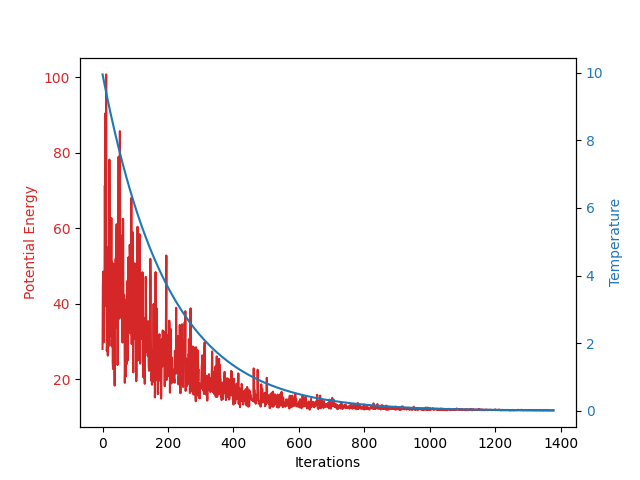
\includegraphics[width=\linewidth]{images/Figure1.N5.png}
    \caption{Potential Energy and Temperature over Iterations}
    \label{fig:Figure1.N5.png}
\end{figure}
\noindent We can easily appreciate that the value of the potential energy tends rapidly toward the optimal value.
\clearpage
\noindent In the \autoref{fig:Figure2.N5.png} we have plotted the snapshot of the optimal configuration for $N=5$ charges.
\begin{figure}[H]
    \centering
    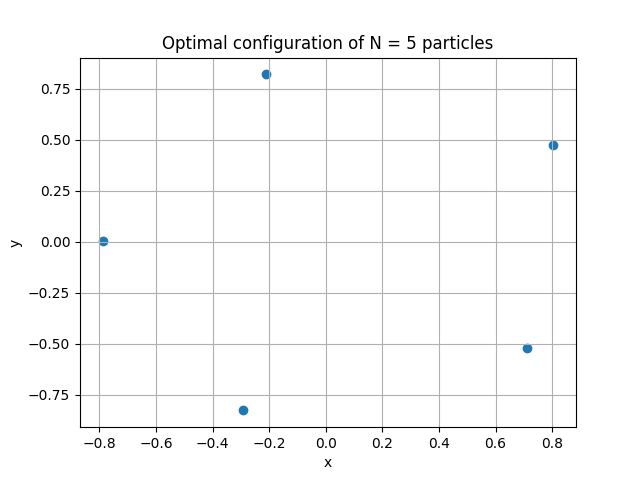
\includegraphics[width=\linewidth]{images/Figure2.N5.png}
    \caption{}
    \label{fig:Figure2.N5.png}
\end{figure}
\noindent 
As we can see the charges lies on a single shells centred in $(0,0)$, forming a pretty regular pentagon. \\\\
We have computed the average value of the last 100 iteration, the value of the potential energy at the optimal configuration is: $\Tilde{E}_{opt}=11.7453$. The absolute minimum energy value found in an iteration is $E_{min}=11.7046$.\\\\

\clearpage
\section{Results - \textit{N=20}}
We simulate a system of $N=20$ charges with the following parameters:
\begin{itemize}
    \item Start temperature: $T_0=10$
    \item Final temperature: $T_f=0.01$
    \item Temperature step: $\delta_T=0.995$
    \item Displacement amplitude: $\Delta t=0.5$
    \item Monte Carlo iterations for each temperature step: $N_{iter}=10000$
\end{itemize}
For $N=20$ particles, the total energy should be $ \Tilde{E}\approx7.94961\cdot N=158.922
$ and the particles should be in tree shell structure, in particular $N_1=1,N_2=7,N_3=12$.\\\\
In the \autoref{fig:Figure1.N20.png} we have plotted the energy dependence during iterations and the temperature.
\begin{figure}[H]
    \centering
    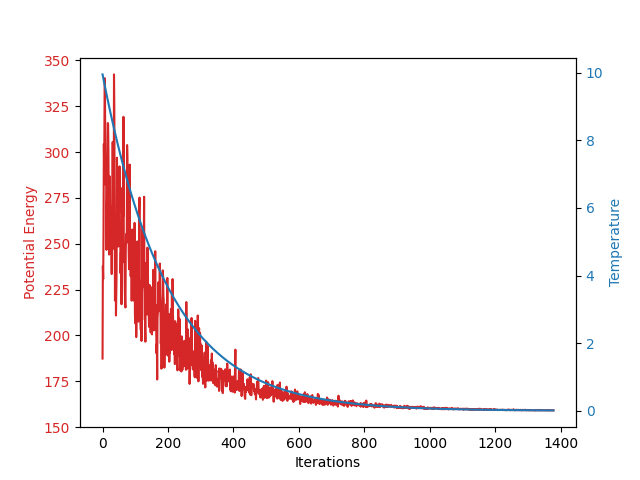
\includegraphics[width=\linewidth]{images/Figure1.N20.png}
    \caption{Potential Energy and Temperature over Iterations}
    \label{fig:Figure1.N20.png}
\end{figure}
\noindent Again, we appreciate that the value of the potential energy tends rapidly toward the optimal value.
\clearpage
\noindent In the \autoref{fig:Figure2.N20.png} we have plotted the snapshot of the optimal configuration for $N=20$ charges.
\begin{figure}[H]
    \centering
    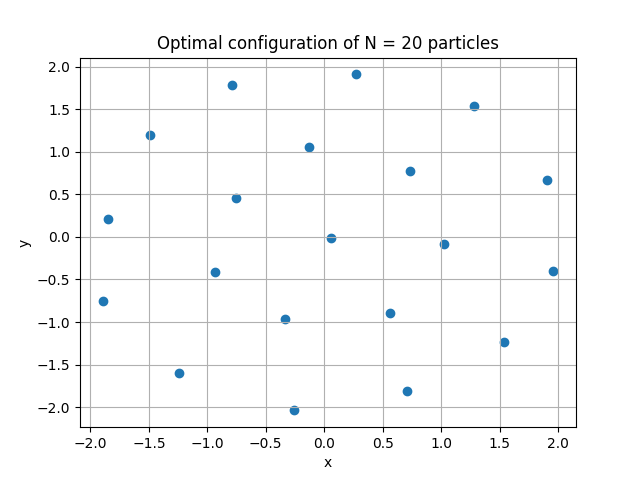
\includegraphics[width=\linewidth]{images/Figure2.N20.png}
    \caption{}
    \label{fig:Figure2.N20.png}
\end{figure}
\noindent As we can see, the charges are arranged in a double-shell configuration centred at $(0,0)$. As expected, at the centre, there is only one charge, while the first shell contains 7 charges, and the second shell contains 12 charges. Together, they form a more complex yet still regular structure.\\\\
Moreover, we have computed the average value of the last 100 iterations. The value of the potential energy at the optimal configuration is $\tilde{E}_{\text{opt}} = 159.2435$. Additionally, the absolute minimum energy value found in any single iteration is $E_{\text{min}} = 159.1289$. These values provide insights into the stability and convergence of the system.

\clearpage
\section{Results - \textit{N=26}}
We simulate a system of $N=26$ charges with the following parameters:
\begin{itemize}
    \item Start temperature: $T_0=10$
    \item Final temperature: $T_f=0.01$
    \item Temperature step: $\delta_T=0.995$
    \item Displacement amplitude: $\Delta t=0.5$
    \item Monte Carlo iterations for each temperature step: $N_{iter}=10000$
\end{itemize}
For $N=26$ particles, the total energy should be $ \Tilde{E}\approx9.76273\cdot N=253.831
$ and the particles should be in tree shell structure, in particular $N_1=3,N_2=9,N_3=14$.\\\\
In the \autoref{fig:Figure1.N26.png} we have plotted the energy dependence during iterations and the temperature.
\begin{figure}[H]
    \centering
    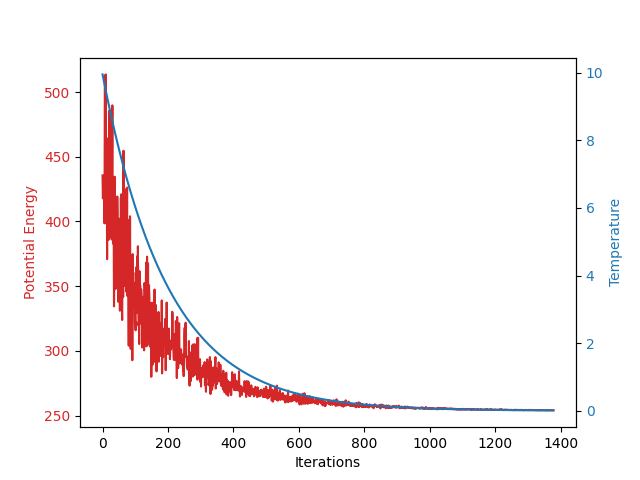
\includegraphics[width=\linewidth]{images/Figure1.N26.png}
    \caption{Potential Energy and Temperature over Iterations}
    \label{fig:Figure1.N26.png}
\end{figure}
\noindent Again, we appreciate that the value of the potential energy tends rapidly toward the optimal value.
\clearpage
\noindent In the \autoref{fig:Figure2.N26.png} we have plotted the snapshot of the optimal configuration for $N=26$ charges.
\begin{figure}[H]
    \centering
    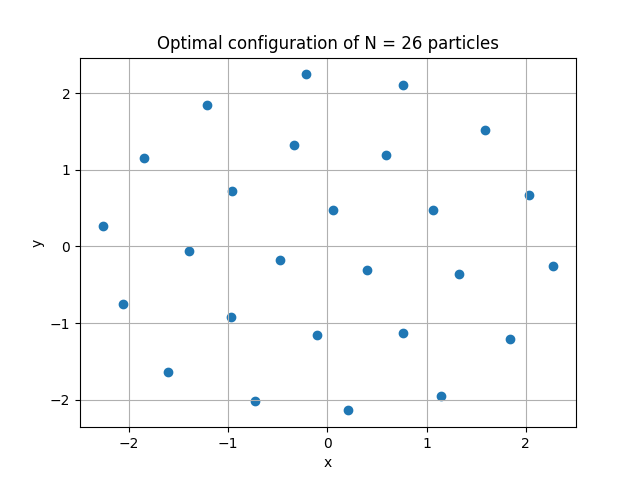
\includegraphics[width=\linewidth]{images/Figure2.N26.png}
    \caption{}
    \label{fig:Figure2.N26.png}
\end{figure}
\noindent We can  appreciate that the charges are arranged in a double-shell configuration centred at $(0,0)$. As expected, at the centre, there are 3 charges, while the first shell contains 9 charges, and the second shell contains 14 charges. Together, they form a more complex yet still regular structure.\\\\We have computed the average value of the last 100 iteration, the value of the potential energy at the optimal configuration is: $\Tilde{E}_{opt}=254.1798$. The absolute minimum energy value found in an iteration is $E_{min}=254.1061$.
\clearpage
\section{Conclusions}
We compare in \autoref{tab:1} the obtained results with the one provided in the literature.
\begin{table}[H]
    \centering
    \begin{tabular}{|c|c|c|}
        \hline
        $N$& Simulations & Literature \\
        &$E/N$ & $E/N$ \\\hline\hline
        5 & 2.3491 & 2.33845 \\\hline
        20 & 7.9622 & 7.94961 \\\hline
        26 & 9.7761 & 9.76273 \\\hline
    \end{tabular}
    \caption{Comparing obtained results with reference data}
    \label{tab:1}
\end{table}
\noindent In \autoref{fig:FigureOCCShells.png} we illustrates the average distance of particles within each defined region (shell) for different configurations. We report the occupation of each shell in \autoref{tab:2}.
\begin{figure}[H]
    \centering
    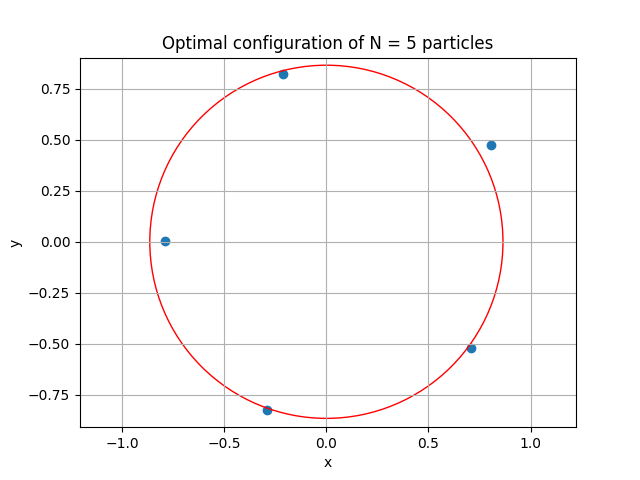
\includegraphics[width=0.495\linewidth]{images/Figure_5.png}
    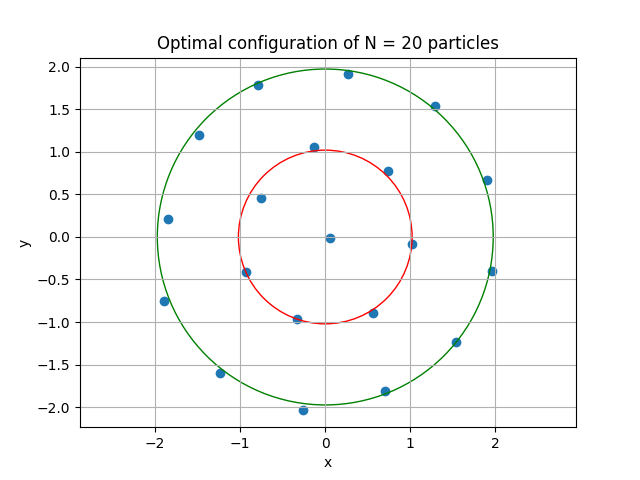
\includegraphics[width=0.495\linewidth]{images/Figure_20.png}
    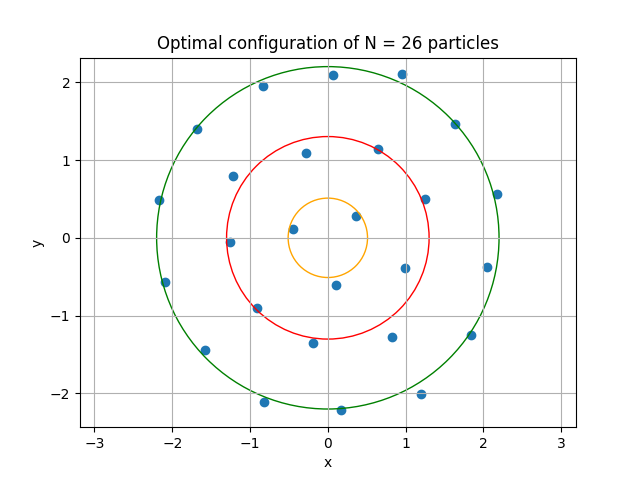
\includegraphics[width=0.495\linewidth]{images/Figure_26.png}
    \caption{Shell occupation for different configurations}
    \label{fig:FigureOCCShells.png}
\end{figure}
\begin{table}[H]
    \centering
    \begin{tabular}{|c|c|c|c|}
        \hline
        $N$& $N_1$ & $N_2$ & $N_3$ \\\hline\hline
        5 & 5 & . & . \\\hline
        20 & 1 & 7 & 12\\\hline
        26 & 3 & 9 & 14 \\\hline
    \end{tabular}
    \caption{Occupation of shells for different configurations}
    \label{tab:2}
\end{table}
\end{document}
